% Chapter 3

\chapter{无人机系统}
\section{系统硬件模块}
\subsection{整体硬件框架}
无人车系统是利用RoboMasters步兵车的底盘搭建的,系统的硬件由控制主板、机载电脑、传感器和外设四部分组成。其中控制主板为RM开发板,主要用于直接无人车,包含STM32微控制器、串行通讯接口(与机载电脑和遥控器的接收机通讯)、CAN通讯接口(与电机集成电调等模块通讯)、多路PWM信号输出接口(用于控制无刷电机转速)等;机载电脑是NVIDIA的Jetson TX2,主要用来执行建图和导航任务,包含ARM架构多核处理器(运行建图、导航等算法)、串行通讯接口(与控制主板通讯)、USB接口(用于连接蓝牙串口模块和鼠标、键盘等设备)等;传感器包括激光雷达(获取点云数据)、GPS模块(测量无人车的初始经纬度坐标)、姿态传感器(测量无人车的航向)、编码器(测量无人车的位移和速度)等;外设包括蓝牙串口模块(与无人机通讯)、遥控装置(用于设置无人车控制模式以及手动控制无人车)等。图~\ref{fig:3-1}为无人车系统的实物图,图~\ref{fig:3-2}为系统的整体硬件框架。

\clearpage 	
\begin{figure}[htb]
	\centering
	\begin{minipage}[t]{\linewidth} 
		\centering
		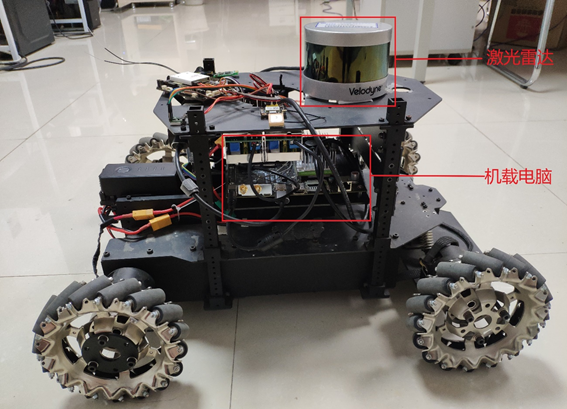
\includegraphics[width=1\columnwidth]{figures/3-1a.png} 
		\subcaption{无人车系统实物图1} 
		\label{fig:3-1a}
	\end{minipage}
	\begin{minipage}[t]{\linewidth} 
		\centering
		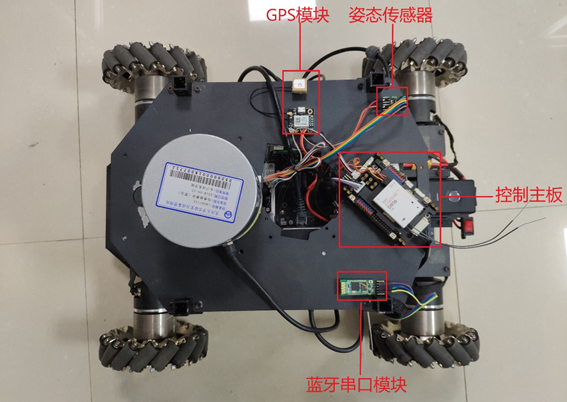
\includegraphics[width=1\columnwidth]{figures/3-1b.png} 
		\subcaption{无人车系统实物图2} 
		\label{fig:3-1b} 
	\end{minipage}
	\caption{无人车系统实物图}
	\label{fig:3-1}
\end{figure}

\clearpage 
\begin{figure}[htb]
	\centering
	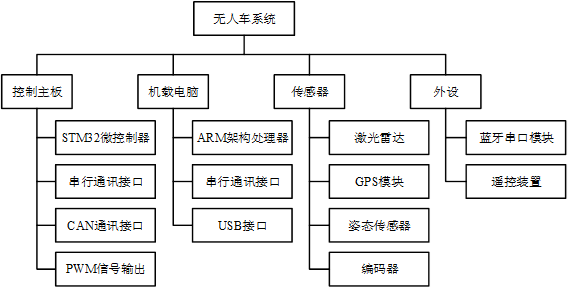
\includegraphics[width=\linewidth]{figures/3-2.png}
	\caption{无人车系统整体硬件框架}
	\label{fig:3-2}
\end{figure}

\subsection{控制主板}
控制主板采用DJI开发的RM开发板。该开发板以高性能的STM32F427IIH6为主控芯片,同时搭载丰富的外设和硬件接口,包含2路CAN口、4路24V电源输出、3路12V电源输出、22路PWM输出、3路串口输出、板载蜂鸣器、板载按键和板载双色LED指示灯~\upcite{r35}。图~\ref{fig:3-3}为该控制主板的外观和主要硬件接口图。

控制主板主要用于接收遥控器或机载电脑发送的运动控制指令,并控制无人车运动,同时将编码器、姿态传感器、GPS模块等测量的数据发送给机载电脑。

\clearpage
\begin{figure}[htb]
	\centering
	\begin{minipage}[t]{0.4\linewidth} 
		\centering
		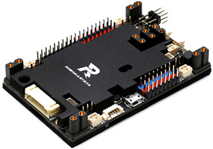
\includegraphics[width=1\columnwidth]{figures/3-3a.png} 
		\subcaption{RM开发板外观} 
		\label{fig:3-3a}
	\end{minipage}
	
	\begin{minipage}[t]{0.6\linewidth} 
		\centering
		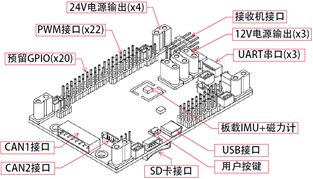
\includegraphics[width=1\columnwidth]{figures/3-3b.png} 
		\subcaption{RM开发板主要硬件接口} 
		\label{fig:3-3b} 
	\end{minipage}
	\caption{RM开发板~\upcite{r35}}
	\label{fig:3-3}
\end{figure}

\subsection{机载电脑}
机载电脑采用NVIDIA英伟达公司推出的Jetson TX2板卡,它是一台基于NVIDIA Pascal$^{TM}$架构的AI单模块超级计算机,拥有256颗CUDA的 GPU 和2颗CPU,内存为 8GB的 LPDDR4,拥有USB、PCIE、Ethernet、HDMI等一系列接口。图~\ref{fig:3-4}为机载电脑Jetson TX2的外观图。

本设计中机载电脑主要用于执行建图和导航算法。首先通过蓝牙串口模块接收无人机发送的目标经纬度坐标数据,然后通过建图和导航算法规划路径,控制无人车安全行驶到目标处。

\clearpage
\begin{figure}[htb]
	\centering
	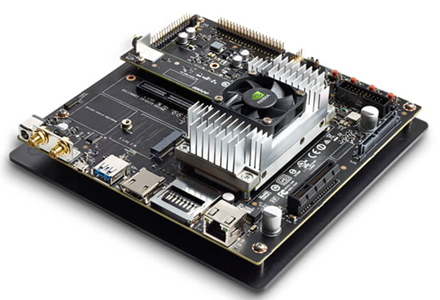
\includegraphics[width=0.6\linewidth]{figures/3-4.png}
	\caption{机载电脑Jetson TX2}
	\label{fig:3-4}
\end{figure}

\subsection{激光雷达}
激光雷达采用Velodyne公司研发的Velodyne VLP-16 3D激光雷达。该激光雷达拥有360°水平视场角以及30°垂直视场角,垂直方向拥有16线激光,支持360度全覆盖3D激光扫描,拥有近300000点/秒的高速激光测距采样速率,测量距离长达100米,精确度达到±3cm。同时集成有Web服务器,可方便地进行监控和配置。图~\ref{fig:3-5}为该激光雷达的外观图。

本设计中主要利用激光雷达获取点云数据,再利用点云数据进行建图、避障和导航。同时由于编码器测量的位移和速度具有累积误差,因此可以使用点云数据辅助定位。

\begin{figure}[htb]
	\centering
	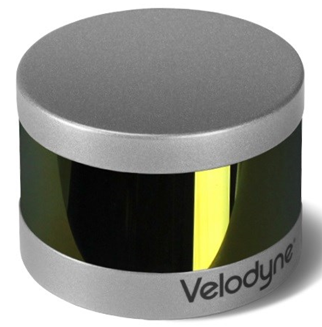
\includegraphics[width=0.5\linewidth]{figures/3-5.png}
	\caption{Velodyne VLP-16 3D激光雷达}
	\label{fig:3-5}
\end{figure}

\subsection{GPS模块}
GPS模块采用GT-U7 GPS模块,该GPS模块具有高灵敏度、低功耗、小型化等优点,定位精度达到2.5m。本设计中,无人车系统中的GPS模块用于获取无人车初始位置的GPS坐标,从而解算出目标在无人车坐标系下的局部坐标。图~\ref{fig:3-6}为GPS模块实物图。

\begin{figure}[htb]
	\centering
	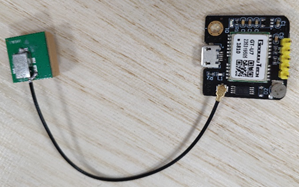
\includegraphics[width=0.4\linewidth]{figures/3-6.png}
	\caption{GT-U7 GPS模块}
	\label{fig:3-6}
\end{figure}

\subsection{姿态传感器}
姿态传感器采用MPU9250模块,该模块内部包含加速度计、陀螺仪和磁力计,可输出三轴加速度、角速度和磁感应强度,同时利用卡尔曼滤波算法,可以解算出高精度的三轴姿态角,姿态测量静态精度达到0.05度,动态精度达到0.1度。该模块支持UART和I$^2$C两种接口,同时可以通过UART接口接收符合NMEA-0183标准的GPS数据。

本设计中,GPS模块与MPU9250模块通过串口相连,GPS数据先传输给MPU-9250模块,然后与加速度、姿态等数据一并传输给控制主板。图~\ref{fig:3-7}为MPU9250姿态传感器实物图。

\begin{figure}[htb]
	\centering
	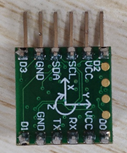
\includegraphics[width=0.3\linewidth]{figures/3-7.png}
	\caption{MPU9250姿态传感器}
	\label{fig:3-7}
\end{figure}

\subsection{编码器}
编码器采用无人车地盘RM电机内部集成的编码器,该编码器可以输出电机的角度,通过差分可以求出电机的速度,再利用麦克纳姆四轮全向底盘的运动学传输方程,可以推算出无人车运动的位移和速度。

\subsection{蓝牙串口模块}
蓝牙串口模块选用HC-05主从一体蓝牙串口模块,与无人机系统一致。本项目中无人车端的蓝牙串口模块用于接收无人机端蓝牙串口模块发送的目标经纬度坐标数据。

\subsection{遥控装置}
遥控装置使用DJI生产的DR16接收机+DT7遥控器组成的遥控系统。该遥控器工作于2.4GHz频段,采用DBUS协议,具有长达1000米的通信距离。图~\ref{fig:3-8}为该遥控装置实物图。

本设计中遥控器可用于手动控制无人车运动,以及切换无人车控制模式。

\begin{figure}[htb]
	\centering
	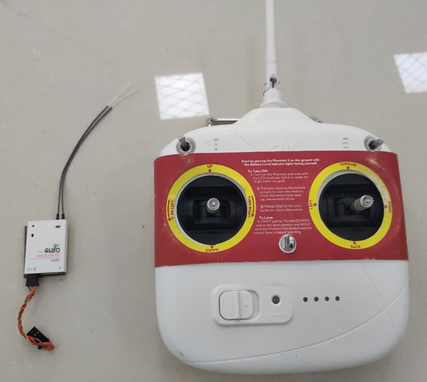
\includegraphics[width=0.8\linewidth]{figures/3-8.png}
	\caption{DR16接收机和DT7遥控器}
	\label{fig:3-8}
\end{figure}

\section{自主定位}
进行自主定位时,无人车系统的坐标系设定如图~\ref{fig:3-9}所示。其中,$O-x-y$为局部坐标系,以无人车起点为原点,$x$轴指向北,$y$轴向左。$O'-x'-y'$为车身坐标系,以无人车中心为原点,车身朝向为$x'$轴,$y'$轴向左。$x'$轴与$x$轴夹角即为偏航角$yaw$。

\begin{figure}[htb]
	\centering
	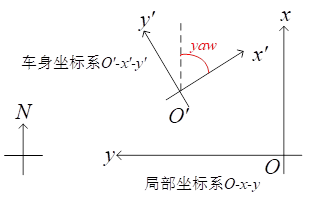
\includegraphics[width=0.6\linewidth]{figures/3-9.png}
	\caption{局部坐标系与车身坐标系}
	\label{fig:3-9}
\end{figure}

本设计中无人车的自主定位基于里程计和激光雷达实现,类似于视觉惯性里程计,只是这里使用激光雷达代替了视觉传感器。

里程计包括无人车在局部坐标系下的位置($x$、$y$坐标和偏航角$yaw$)和车身坐标系下的速度($x'$、$y'$速度和$yaw$角速度)信息,通过编码器和姿态传感器获得,其中编码器可以提供无人车在车身坐标系下的位移和度,姿态传感器可以提供无人车的偏航角及其角速度,利用运动学方程可以计算得到里程计。由于里程计是利用编码器实现的,因此轮子发生打滑将会产生累积误差。另外姿态传感器如果利用磁力计计算偏航角,则容易受到磁场干扰,如果利用角速度积分计算偏航角,则会有累积误差。

利用激光雷达也可以实现无人车的定位,通过激光雷达扫描数据前后2帧数据之间的匹配可以估计出无人车的运动信息,但存在噪声引起的累积误差,也会导致里程计漂移。因此可以将里程计数据与激光雷达扫描数据融合,估计出更为精准的无人车位置信息。

本设计利用ROS的laser\_scan\_matcher包来实现无人车的精确定位。laser\_scan\_matcher是基于Andrea Censi的CSM (Canonical Scan Matcher)算法\upcite{r36}实现的一种增量式激光匹配器,相较于传统的帧与帧之间的匹配,该匹配器利用关键帧进行匹配,可以有效抑制噪声引起的累积误差。同时该匹配器还可以输入IMU、里程计等数据,提供对激光雷达传感器当前位置的猜测,可以加速匹配过程并提高定位精度。

\section{SLAM建图}
本设计使用基于激光雷达的SLAM,即激光SLAM\upcite{r37},相较于视觉SLAM\upcite{r38, r39},优点是建图精度高,生成的占据栅格地图(occupancy grid maps)特别适合进行路径规划。缺点是较为缺乏回环检测能力,累积误差消除较为困难。

在ROS中常用的激光SLAM算法有Gmapping\upcite{r40, r41}、HectorSLAM\upcite{r42}、Cartographe\upcite{r43}等等,这些算法各自具有其优缺点:

\begin{enumerate}[label=(\arabic*)] 
	\item Gmapping算法。Gmapping是基于滤波框架的SLAM,有效利用了里程计信息来提供机器人的位姿先验,因此对激光雷达频率要求低,适用于构建小场景地图。缺点是依赖里程计,无法适用于无人机以及地面小车在不平坦区域建图,并且没有回环检测,在回环闭合时可能造成地图错位;
	\item HectorSLAM算法。不需要使用里程计,可用于空中无人机以及地面小车在不平坦区域建图。缺点是要求激光雷达的更新频率较高、测量噪声小,在机器人快速转向时容易发生错误匹配,导致建出的地图发生错位;
	\item Cartographer算法。Cartographer是基于优化框架的SLAM,具有回环检测,因此建图精度高,可用于构建大场景地图,同时不需要使用里程计,适用于手持激光雷达完成SLAM过程。缺点是图优化计算量大。
\end{enumerate}

通过对比上述3种常用激光SLAM算法,本设计选择了最为合适的Gmapping算法。Gmapping算法基于Rao-Blackwellized粒子滤波(RBPF)算法\upcite{r44},在RBPF算法基础上做了两点改进:改进建议分布和选择性重采样\upcite{r40}。其定位与建图的过程分为4步:采样、计算重要性权值、重采样、地图估计。

\section{自主导航}
自主导航采用ROS中的navigation包,图~\ref{fig:3-10}为navigation导航包的整体框架。其中,move\_base模块为整个导航算法的核心,它包含了以下5个模块:

\begin{enumerate}[label=(\arabic*)] 
	\item 全局代价地图。用于全局路径规划,由外部提供的地图和激光雷达点云数据计算得到,基本上不会更新,一般是静态costmap类型;
	\item 局部代价地图。用于局部路径规划,由激光雷达点云数据计算得到,实时更新;
	\item 修复机制。包括rotate\_recovery和clear\_cost\_map\_recovery,用于机器人不能找到路径时进行修复;
	\item 全局路径规划器。依据全局代价地图,利用全局路径规划算法,生成机器人到目标位置的全局路径。导航包提供了2种全局路径规划算法,分别是Dijkstra算法\upcite{r45}和A*算法\upcite{r46},默认使用Dijkstra算法;
	\item 局部路径规划器。依据局部代价地图、全局路径规划器生成的全局路径和机器人的定位信息,利用局部路径规划算法,生成机器人到达目标位置的局部路径,并输出控制机器人运动的速度命令。由于局部代价地图是实时更新的,因此局部路径也是实时更新的,而机器人按照局部路径运动,并非全局路径,因此可以实现动态避障。导航包提供了多种局部路径规划器,包括dwa\upcite{r47}、trajectory、teb\upcite{r48, r49}、eban\upcite{r50}等等。
\end{enumerate}

当一条全局路径导航失败时,全局路径规划器会尝试生成新的全局路径,如果不能生成可行的全局路径,那么算法会执行修复操作,然后再次尝试生成全局路径,倘若还是无法生成可行的全局路径,则导航失败。

除了move\_base模块,导航包还需要用户提供机器人的定位信息、目标位置信息、激光雷达点云数据和地图。本设计中,定位信息可以由自主定位系统提供,目标位置信息由无人机系统通过检测和定位算法得到,并通过蓝牙发送给无人车,激光雷达点云数据由velodyne包处理激光雷达输出的原始数据得到。地图是可选项,因此导航算法存在3种模式,一是没有地图,进行局部导航,导航效果会差很多;二是事先有地图,直接进行全局导航,但本项目中事先并没有地图,因此该方案不可行;三是利用建图算法生成地图,边建图边导航,虽然效果不及全局导航,但是胜过局部导航,并且方案可行。因此本设计采用边建图边导航的自主导航方式。

\begin{figure}[htb]
	\centering
	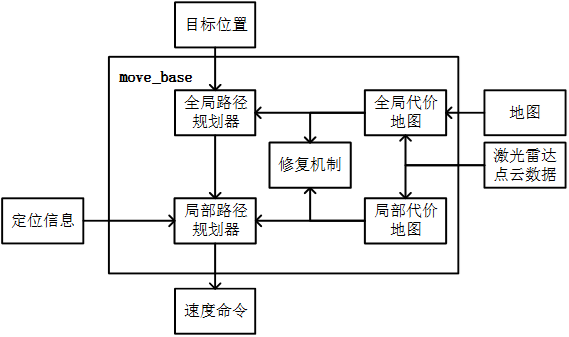
\includegraphics[width=\linewidth]{figures/3-10.png}
	\caption{navigation导航包整体框架}
	\label{fig:3-10}
\end{figure}

\section{系统软件设计}
无人车系统的机载电脑Jetson TX2使用Ubuntu 16.04操作系统,并装有ROS,本项目分别利用ROS的laser\_scan\_matcher包、gmapping包和navigation包实现了无人车的自主定位、SLAM建图和自主导航功能。图~\ref{fig:3-11}为无人车系统的软件流程图,系统首先等待无人机发送目标位置信息,接收到目标位置信息后,启动无人车,开始同步进行定位、建图和导航,无人车达到所有目标位置后,返回其初始位置,搜索任务完成。

\clearpage
\begin{figure}[htb]
	\centering
	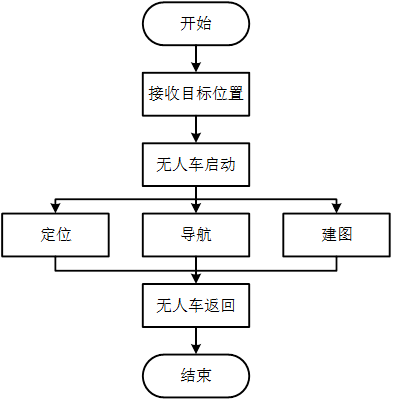
\includegraphics[width=0.8\linewidth]{figures/3-11.png}
	\caption{无人车系统软件流程图}
	\label{fig:3-11}
\end{figure}

\section{本章小结}
本章首先介绍了无人车系统的硬件框架和模块,然后依次介绍了如何实现无人车的自主定位、SLAM建图和自主导航,最后介绍了系统的软件设计。


